\documentclass{ctexart}

\title{\Large 555时基电路应用\\{\large 实验报告}}
\author{\large  信息科学技术学院 \quad 吴海\MyFont{垚} PB22051035 \\\large  信息科学技术学院 \quad 李\quad 毅 PB22051031 \\{教室:电四楼112室\quad 座位号:12}}
\date{2023年4月8日}
\usepackage{ctex}
\setCJKfamilyfont{myfont}{SimSun.ttf}
\newcommand{\MyFont}{\CJKfamily{myfont}}
\usepackage{amsmath}
\usepackage{amsfonts}
\usepackage{amssymb}
\usepackage{bm}
\usepackage{enumerate}
\usepackage{geometry}
\geometry{left=2.5cm,right=2.5cm,top=2cm,bottom=2cm}
\usepackage{fancyhdr}
\usepackage{lastpage}
\usepackage{booktabs}
\pagestyle{fancy}
\fancyhead[l]{ }
\fancyhead[r]{ }
\fancyhead[C]{
	\begin{tabular}{cclclc}
         & \multicolumn{4}{c }{\textbf{555时基电路应用 \quad 实验报告}}                                    &            \\
信息科学技术学院 & \multicolumn{2}{c}{PB22051035 吴海\MyFont{垚}} & \multicolumn{2}{c}{PB22051031 李毅} & 2024年4月8日
\end{tabular}
}
\fancyfoot[C]{ 第 {\thepage} 页,共 \pageref{LastPage} 页}
\renewcommand{\headrulewidth}{2pt}
\usepackage{graphicx}
\usepackage{geometry}
\usepackage[hidelinks]{hyperref}
\usepackage{multicol}
\usepackage{multirow}
\usepackage{ragged2e}
\usepackage[square,comma,numbers,super]{natbib}
\bibliographystyle{unsrt}
\usepackage{siunitx}
\usepackage{subfigure}
\usepackage{wrapfig}
\usepackage{xcolor}
\usepackage{cite}
\begin{document}
    \maketitle
    \thispagestyle{empty}
    
    \newpage 
    \setcounter{page}{1}

    \section*{第一部分 \quad 实验目的}

\begin{enumerate}
    \item 掌握555型集成时基电路的结构及工作原理
    \item 掌握555型集成时基电路的基本应用
\end{enumerate}

    \section*{第二部分 \quad 实验原理}
555型集成时基电路是一种产生时间延迟和多种脉冲信号的电路

\subsection*{1.555定时器内部框图及引脚排列}

555定时器内部框图及引脚排列如下图所示:

    \begin{minipage}[c]{\textwidth}
         \centering
         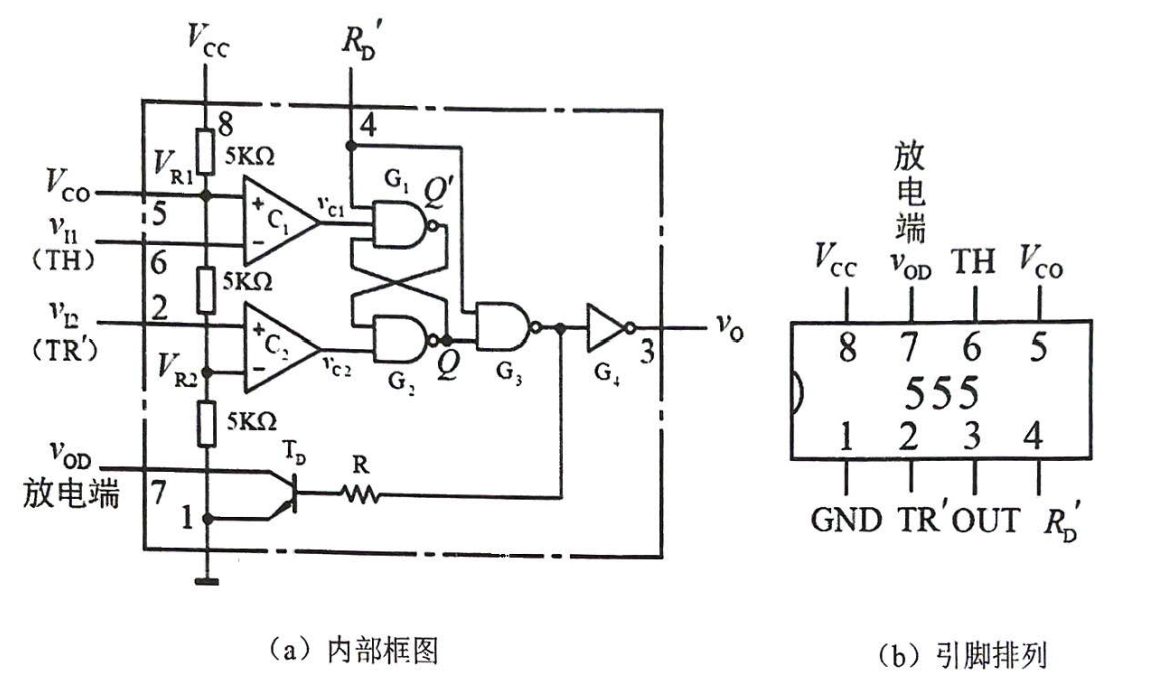
\includegraphics[width=\linewidth]{1.1.png}
        
    \end{minipage}

各引脚功能如下:
\begin{enumerate}[(1)]
    \item 1脚为接地端GND
    \item 2脚为低电平触发端,由此输入低电平触发脉冲
    \item 3脚为输出端, 双极型555输出电流可达200$mA$; CMOS型7555输出电流可达4$mA$
    \item 4脚为复位端,输入负脉冲(或使其电压低于0.7V)可使555定时器直接复位
    \item 5脚为电压控制端,在此端外加电压可以改变比较器的参考电压,不用时,经0.01$\mu F$ 的电容接地,以防止引入干扰;
    \item 6脚为高电平触发端,由此输入高电平触发脉冲
    \item 7脚为放电端,555定时器输出低电平时,放电晶体管$T_D$导通,外接电容元件通过$T_D$放电\item 8脚为电源电压 $V_{CC}$
\end{enumerate}

\subsection*{2.555电路的工作原理}

由555电路的内部框图可见,它包含两个结构完全相同的比较器 $C_1$ 和 $C_2$。$v_{I1}$ 是比较器 $C_1$ 的输入端(也称阈值端,用 $TH$ 表示), $v_{I2}$ 是比较器 $C_2$ 的输入端(也称触发端,用 $TR'$ 表示)。当控制电压输入端 $V_{co}$ 无外加电压时,$C_1$ 和 $C_2$ 的参考电平(电压比较的基准)由三个 $5k\Omega$ 电阻对 $V_{cc}$ 分压决定。可得,$C_1$ 的同相端电平$V_{R1}=\dfrac{2}{3}V_{CC}$,$C_2$反相端电平$V_{R2}=\dfrac{1}{3}V_{CC}$,如果 $V_{co}$ 外加固定电压,则$V_{R1}=V_{CO}$,$V_{R2}=\dfrac{1}{2}V_{CO}$。

$R'_D$ 是置零输入端,只要在 $R'_D$ 端加上低电平,输出 $v_0$ 便立即被置成低电平,不受其他输入端状态的影响。正常工作时必须使 $R'_D$ 端接高电平。

由图可知,当 $V_{I1}>V_{R1}$、$V_{I2}>V_{R2}$ 时,比较器 $C_1$ 的输出$V_{C1}=0$,比较器 $C_2$ 的输出$V_{C2}=0$。$SR$ 锁存器被置 $0$ ($Q=0$), $TD$ 导通,同时定时器输出 $v_O$ 为低电平。

当 $V_{I1}<V_{R1}$、$V_{I2}>V_{R2}$ 时,锁存器的状态保持不变,因而 $T_D$ 和输出 $v_O$ 的状态也保持不变。

当 $V_{I1}<V_{R1}$、$V_{I2}<V_{R2}$ 时,锁存器被置 $1$ ($Q=1$), $v_O=1$ (为高电平),同时 $T_D$ 截止。

当 $V_{I1}>V_{R1}$、$V_{I2}<V_{R2}$ 时,锁存器处于 $Q=Q'=1$ 的状态, $v_O=1$ (为高电平),同时 $T_D$ 截止。

电路中 $T_D$ 的集电极 $V_{OD}$ 端如果经过电阻接到电源上,只要这个电阻的阻值足够大,$v_O$ 为高电平时,$v_{OD}$ 也一定为高电平,$v_O$ 为低电平时,$v_{OD}$ 也一定为低电平。

为了提高电路的带负载能力,555 定时器还在输出端设置了缓冲门 $G_4$,这使得它能承受较大的负载电流(即能提供较大的电流驱动能力)。此外,555 定时器可在很宽的电源电压范围内工作。双极型 555 定时器的电源电压范围为 $5-16V$,可承受的最大负载电流达 $200mA$。CMOS型 $7555$ 定时器的电源电压范围为 $3-18V$,可承受的最大负载电流为 $4mA$。

555定时器电路的应用设计很方便,只要在外部配上几个适当的阻容元件,就可构成单稳态触发器、多谐振荡器以及施密特触发器等脉冲产生与整形电路以及从微秒到数十分钟的延时电路,从而在工业自动控制、定时、仿声和防盗报警等方面有着广泛的应用。


\newpage
    \section*{第三部分 \quad 实验内容}
    \subsection*{1.用555构成单稳态触发器}
    电路和波形如下图所示:
    
    \begin{minipage}[c]{\textwidth}
         \centering
         
         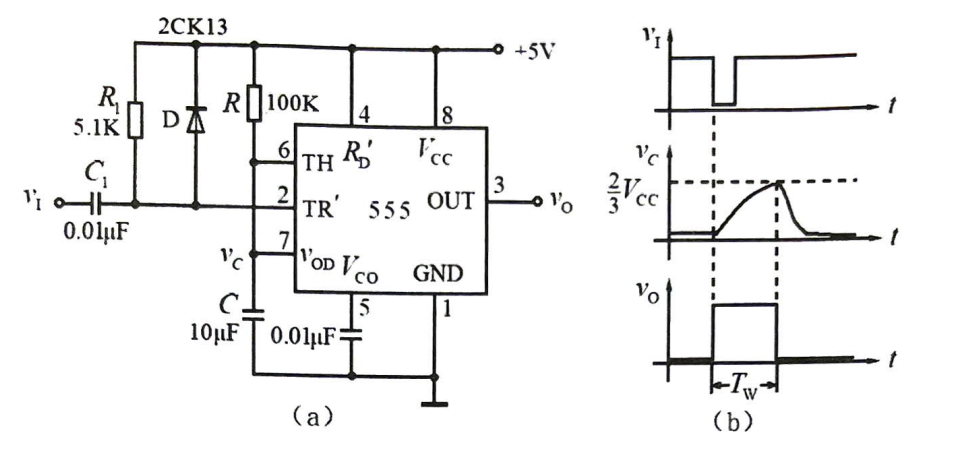
\includegraphics[width=\linewidth]{3.1.1.png}
        
    \end{minipage}

    (1)按如图连线,输入信号$v_I$由单次脉冲源提供负脉冲。用示波器同时观察$V_I,v_c,v_o$波形,测定幅度与暂稳时间。

    实验所观察波形如下图所示:
    
    \begin{figure}[htbp]
        \centering
        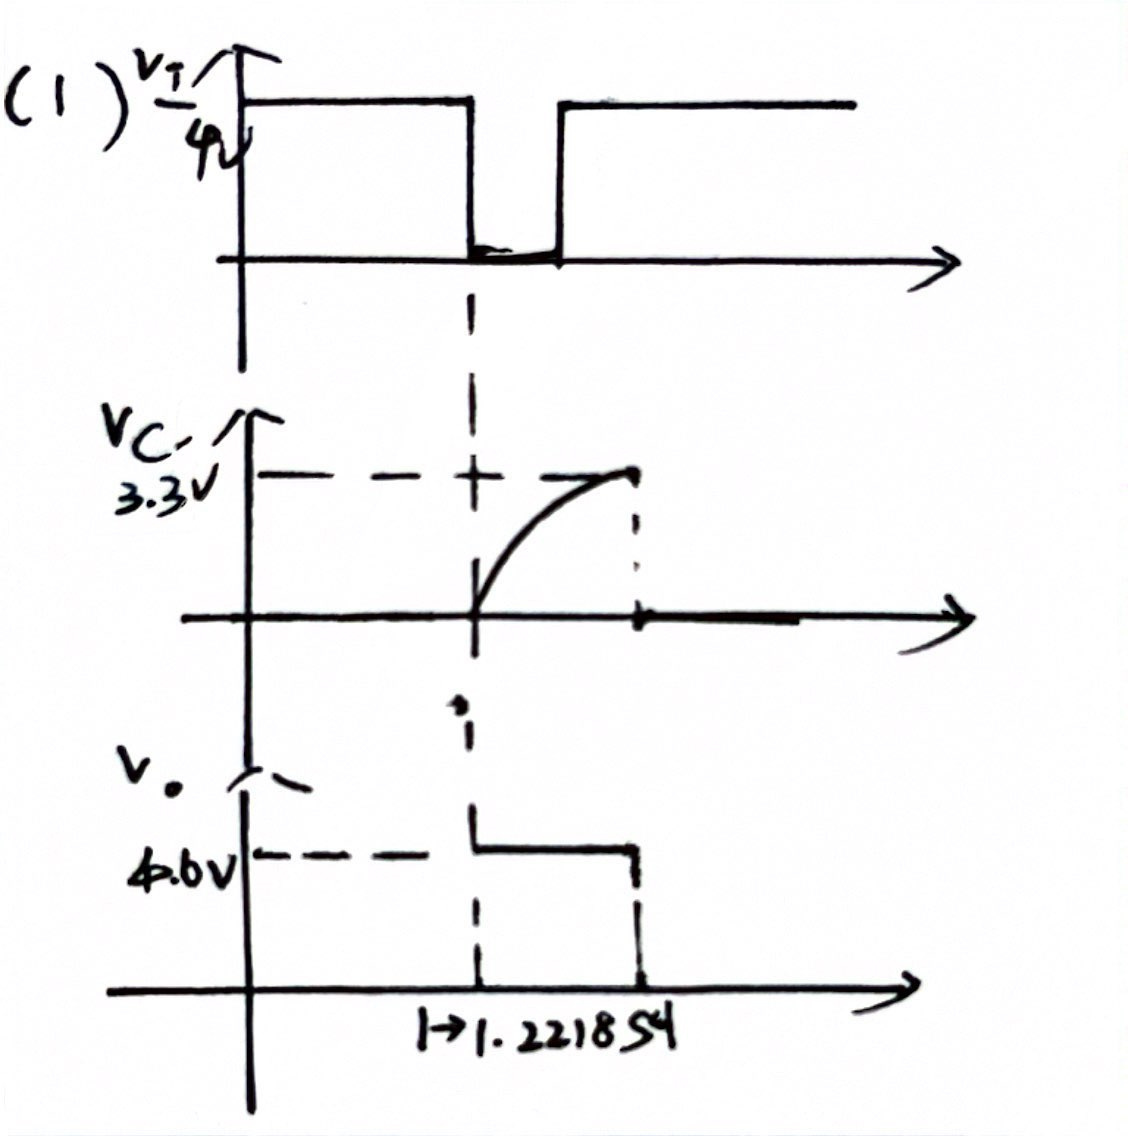
\includegraphics[width=8cm]{3.1.2.jpg}
    \end{figure}

    有图像可知,$v_I$幅度与信号发生器所设置相同,结果理想;

    $v_c$的幅度为3.3V,与理论值$\frac{2}{3}V_{cc}$较为符合,误差不大

    $v_o$的幅度为4.6V,与理论值5V有些偏差,与某些负载有关。其$T_w$为1.2218s。
    
    (2)将R改为10K$\Omega$,C改为0.01$\mu F$输入信号$v_I$加1kHZ连续脉冲,观察$V_I,v_c,v_o$波形,测定幅度与暂稳时间。

    其波形如下图所示:
    
    \begin{figure}[htbp]
        \centering
        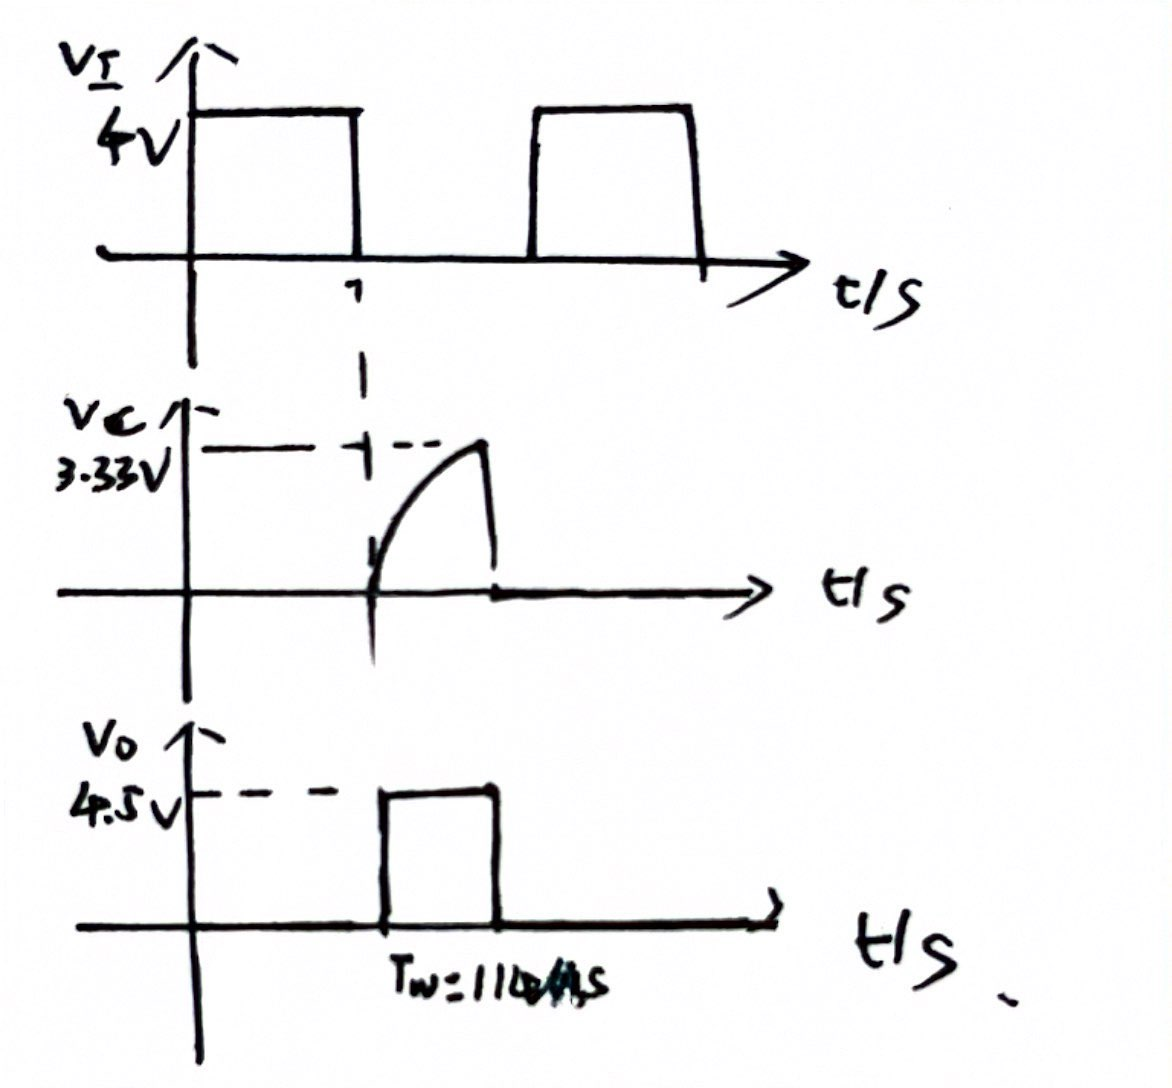
\includegraphics[width=8cm]{3.1.3.jpg}
    \end{figure}



    
    $v_c$的幅度为3.33V,与理论值$\frac{2}{3}V_{cc}$较为符合,误差不大

    $v_o$的幅度为4.5V,与理论值5V有些偏差,与某些负载有关。其$T_w$为114$\mu$s。

    \subsection*{2.用555构成多谐振荡器}
    \begin{minipage}[c]{\textwidth}
         \centering
         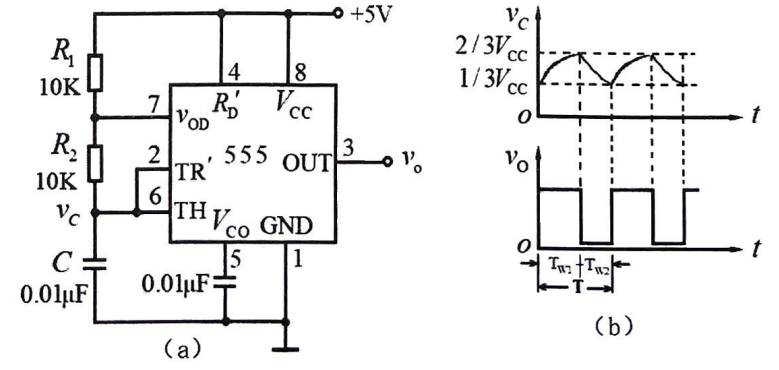
\includegraphics[width=\linewidth]{3.2.1.png}
    \end{minipage}

    (1)如图所示,用555定时器和外接元件$R_1,R_2,C$构成多谐振荡器。电路没有稳态,仅存两个暂稳态,电路亦不需要外加触发信号,仅用电源通过$R_1,R_2$向c充电,以及C用过$R_2$向放电段放电,使电路产生振荡。

    \begin{minipage}[c]{\textwidth}
            \centering
            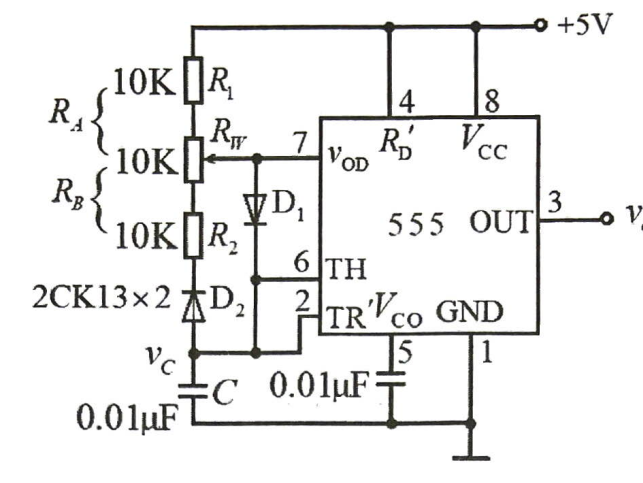
\includegraphics[width=\linewidth]{3.2.2.png}
    \end{minipage}

    所得波形如图所示:
    
    \begin{figure}[htbp]
        \centering
        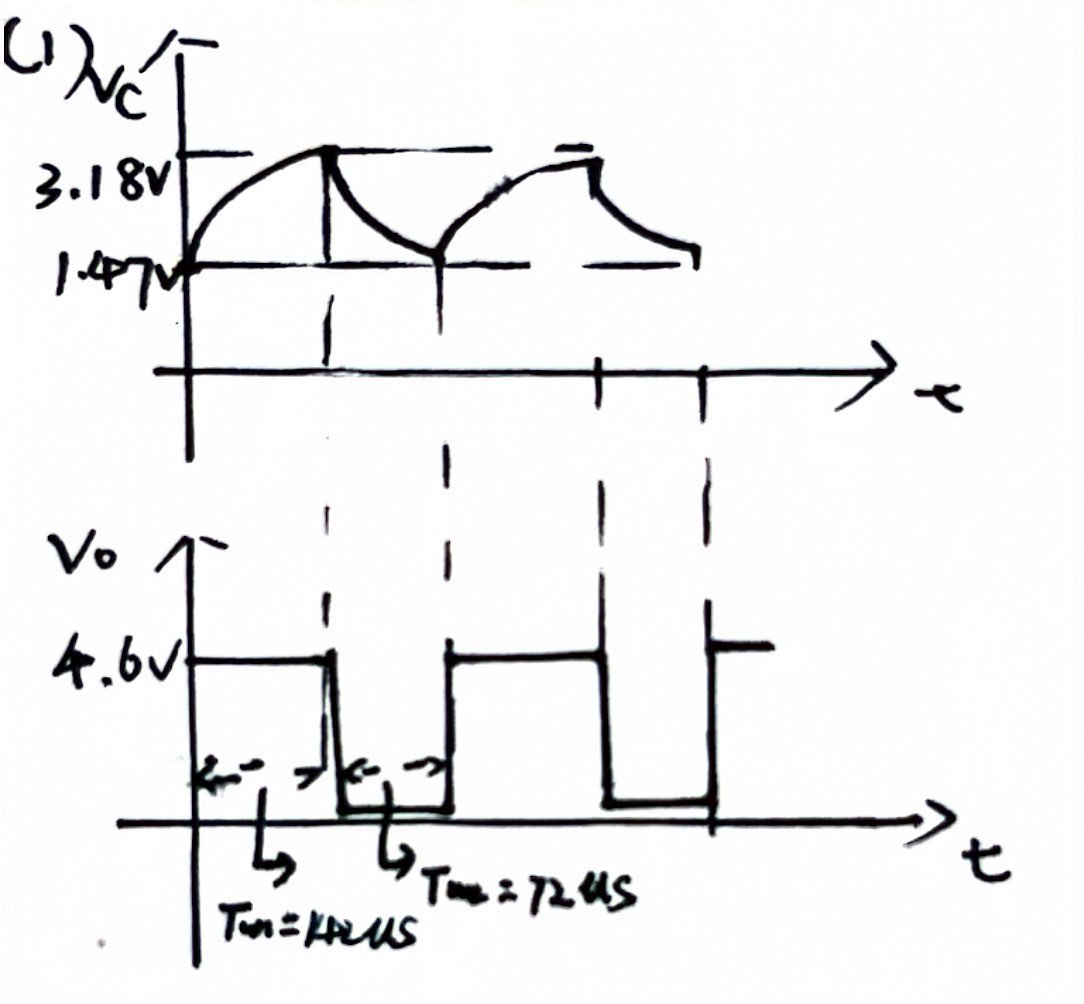
\includegraphics[width=8cm]{3.2.3.jpg}
    \end{figure}

    观察可知,$v_c$的两个对应幅值分别为3.18V,1.47V,与理论值相近。

    $v_0$的幅值为4.6V,$T_{w1}=142\mu s,T_{w2}=72\mu s$,理论值分别对应$T_{w1}=140\mu s,T_{w2}=70\mu s$,结果十分理想。

    (2)按上图连线,组成占空比可调节的多谐振荡器。并调节可变电阻器$R_w$组成占空比为50\%的方波信号发生器,观测并记录$v_c,v_o$波形及参数

    所得波形如图所示:
    
    \begin{figure}[htbp]
        \centering
        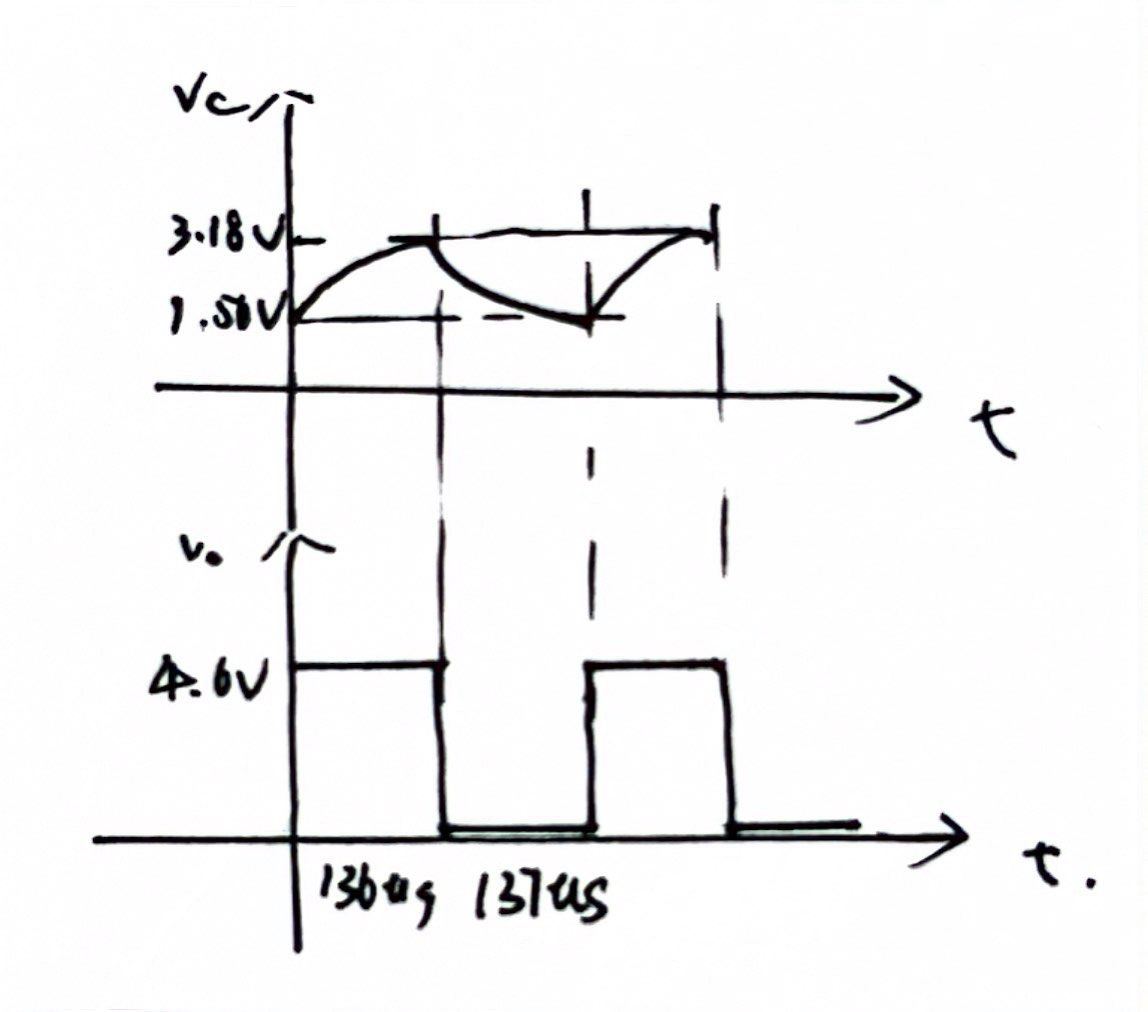
\includegraphics[width=8cm]{3.2.4.jpg}
    \end{figure}
    
    观察可知,$v_c$的两个对应幅值分别为3.18V,1.56V,与理论值相近。

    $v_0$的幅值为4.6V,$T_{w1}=136\mu s,T_{w2}=137\mu s$,与理论值接近。

    \subsection*{3.用555构成施密特触发器}
    按下图连线,输入信号$v_s$为1KHz正弦波,接通电源,逐步加大复制,观察并画出波形。
    
     \begin{minipage}[c]{\textwidth}
            \centering
            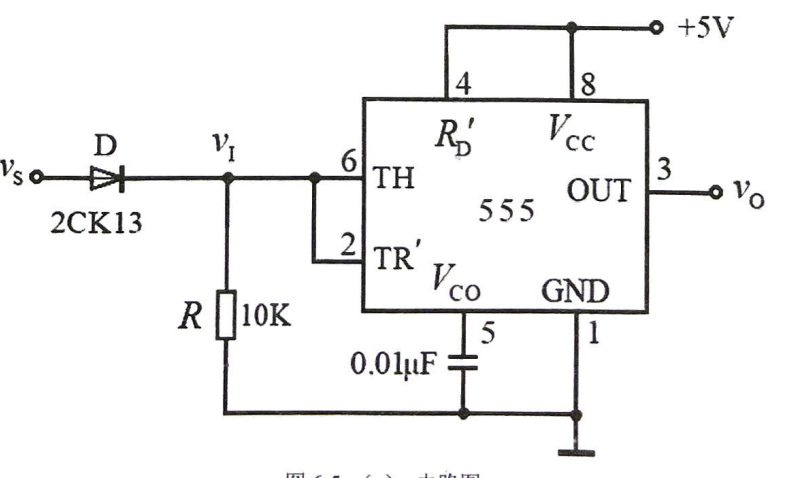
\includegraphics[width=\linewidth]{3.3.1.png}
    \end{minipage}
    
    实验所得波形如图所示:
    
    \begin{minipage}[c]{\textwidth}
            \centering
            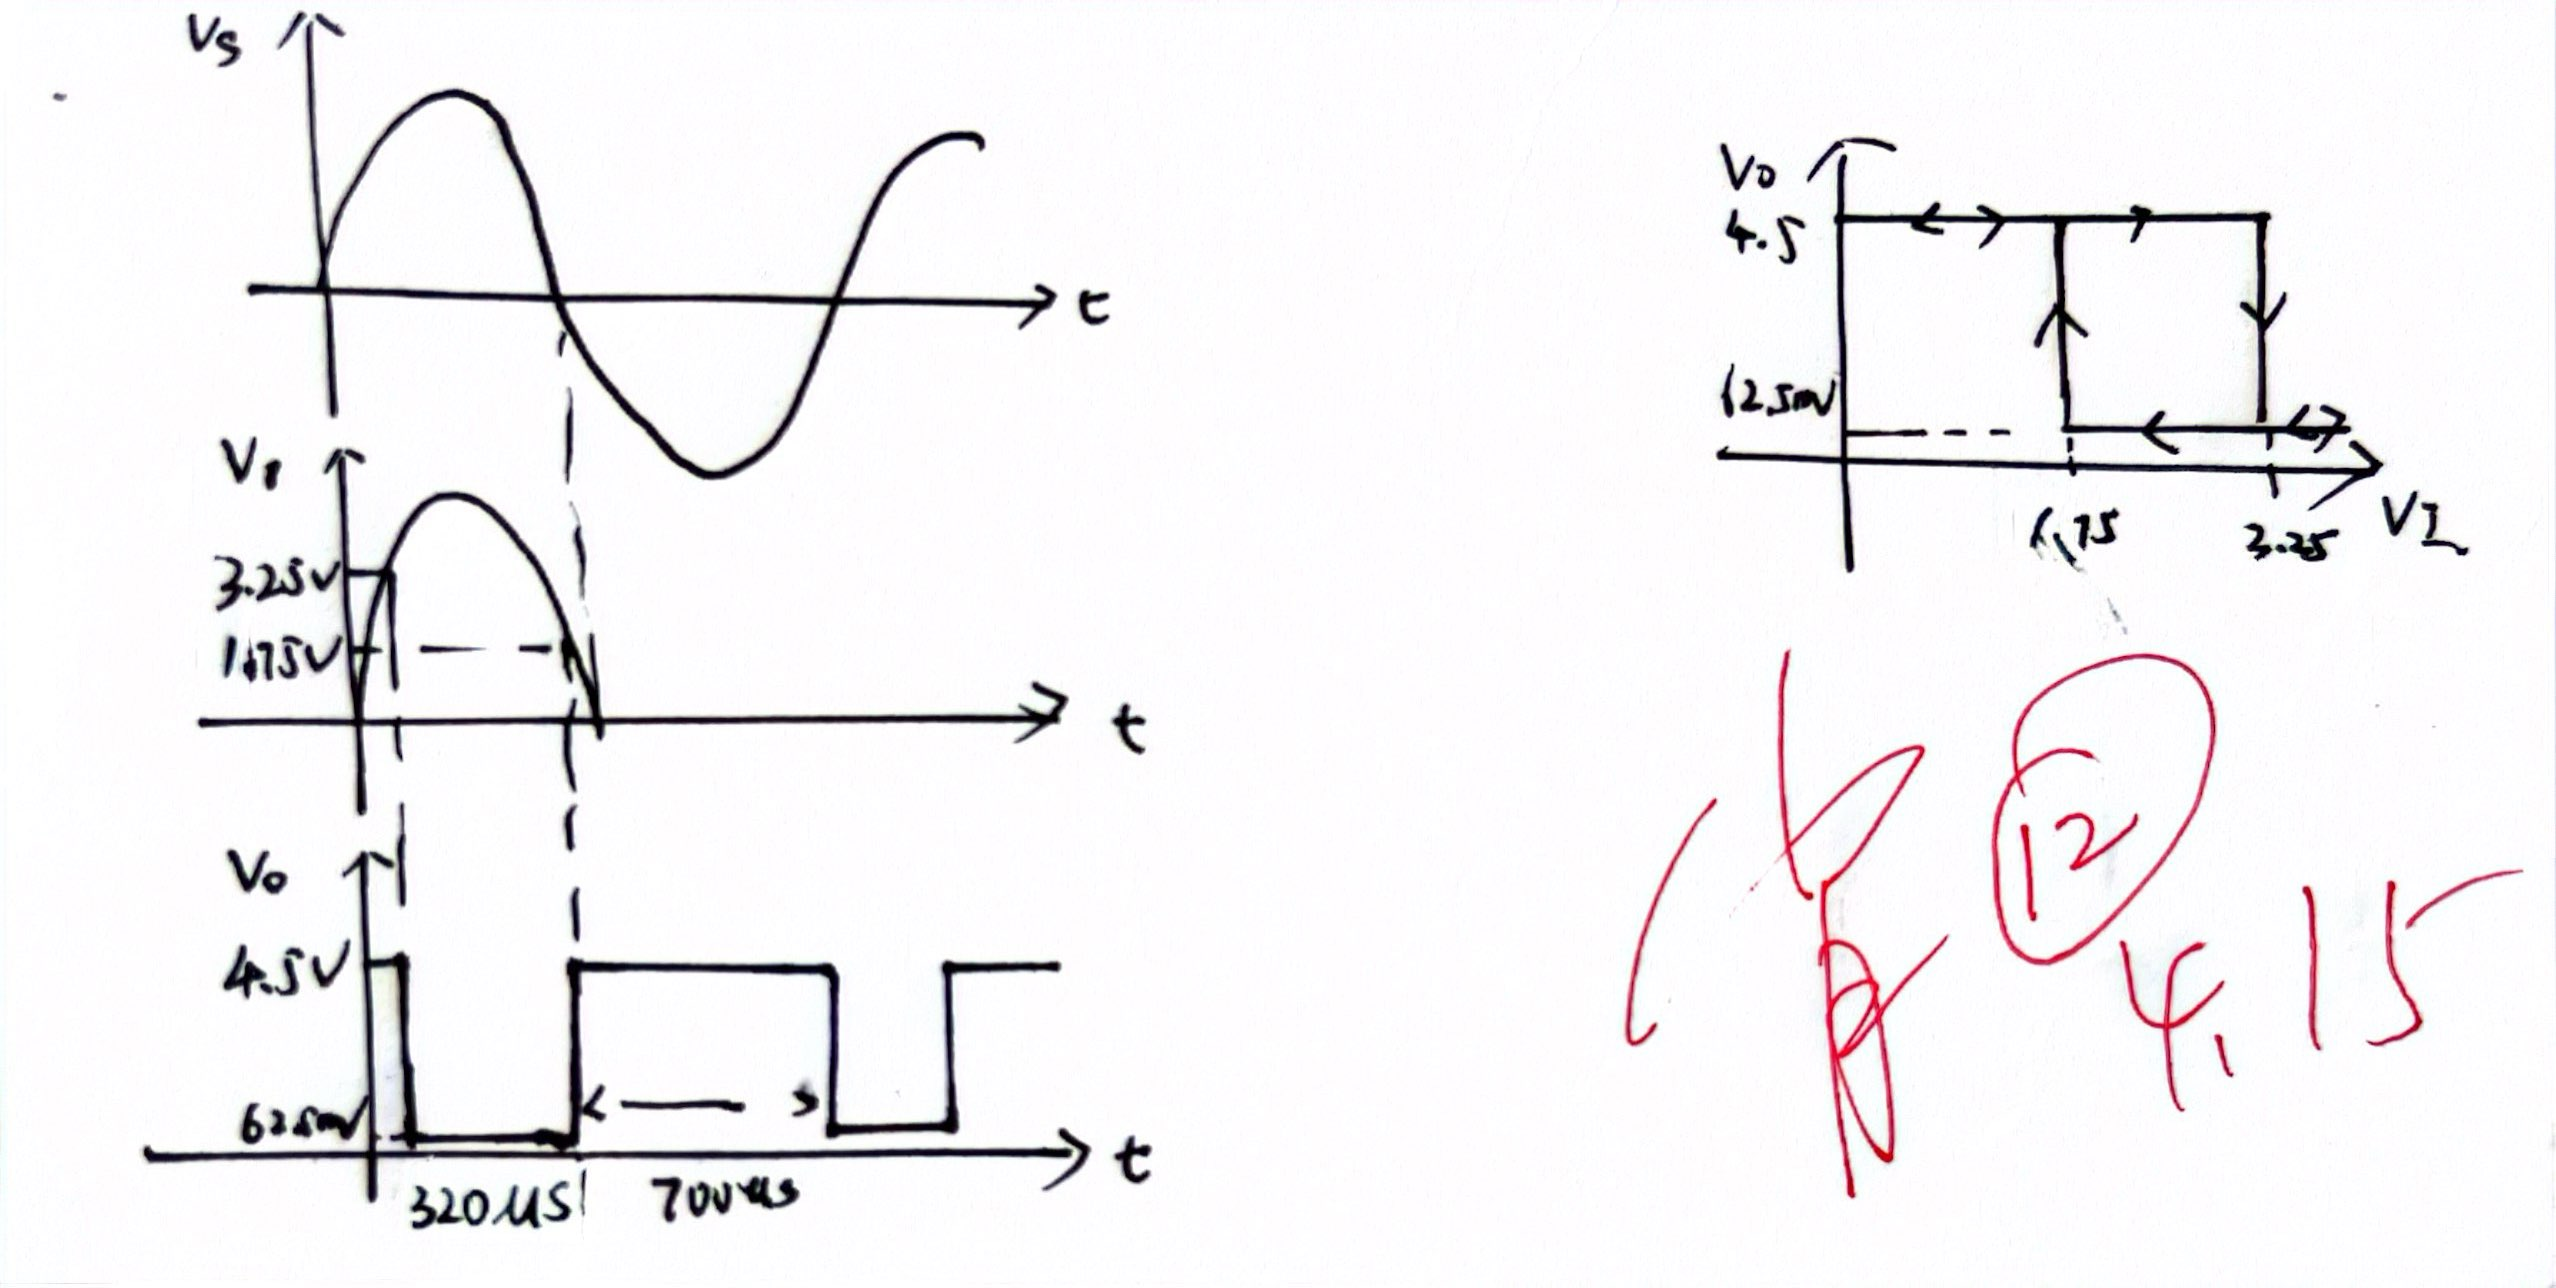
\includegraphics[width=\linewidth]{3.3.2.jpg}
    \end{minipage}

    观察可知,$v_i$的两个对应幅值分别为3.25V,1.75V,与理论值相近。

    $v_0$的幅值为4.5V与62.5mV,$T_{w1}=320\mu s,T_{w2}=700\mu s$,与理论值接近,由上述两波形可画出如图电压传输特征

    


    \section*{第四部分 \quad 思考题}

\subsection*{用555定时器设计一个电子门铃电路并说明其工作原理}

    \begin{minipage}[c]{\textwidth}
            \centering
            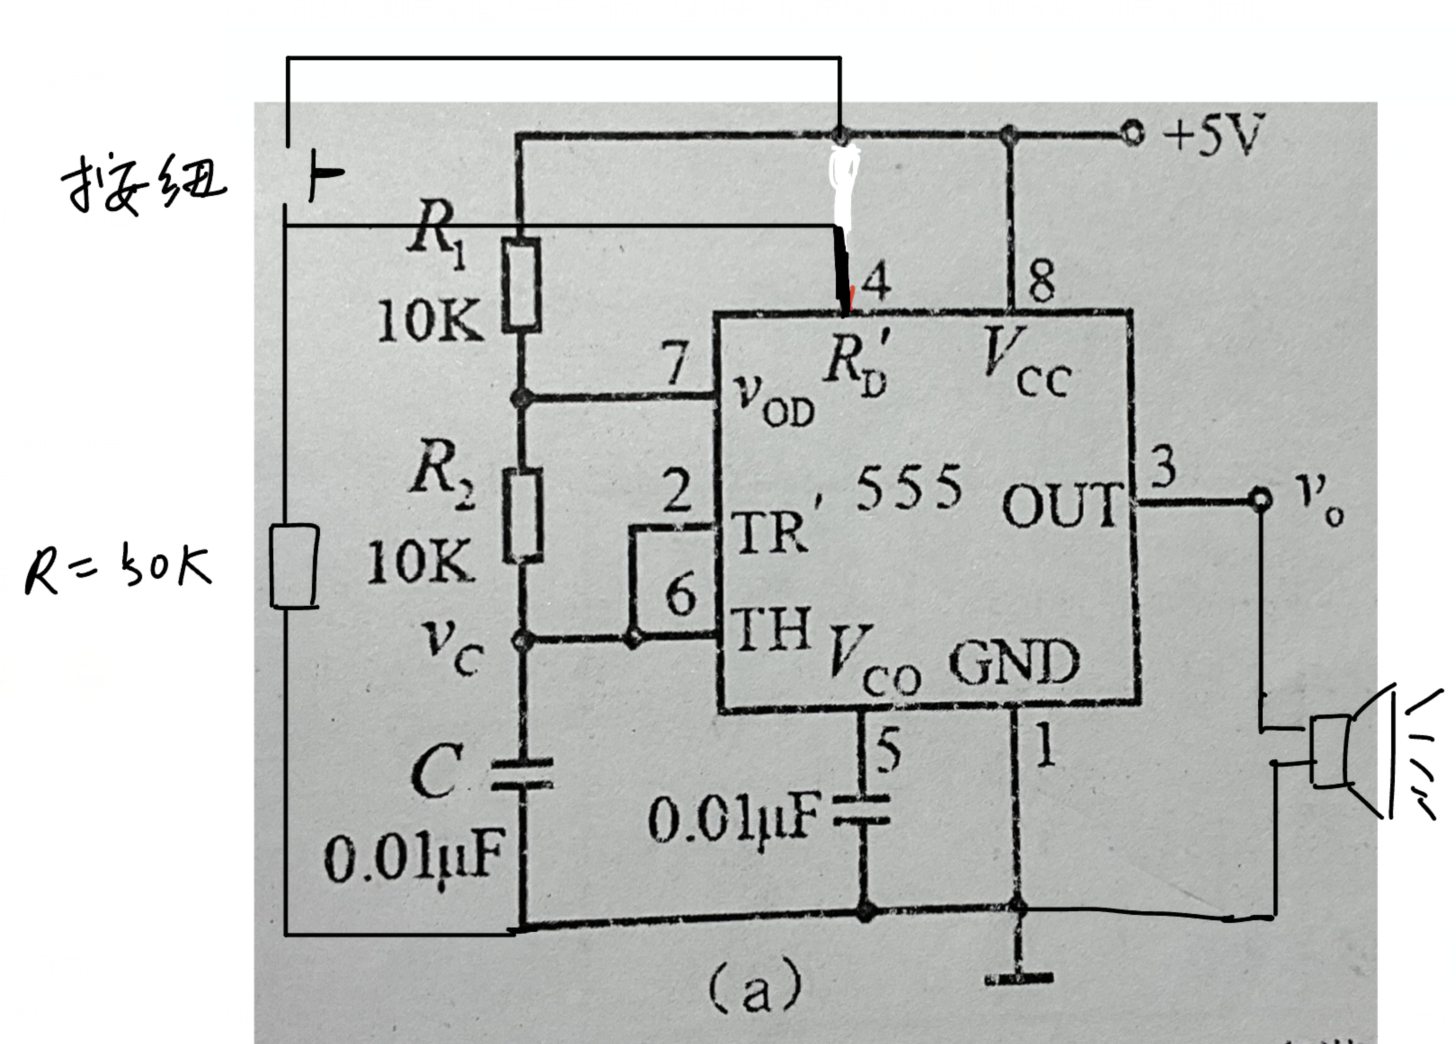
\includegraphics[width=\linewidth]{思考题.png}
    \end{minipage}

~\\

    将实验用多谐振荡电路进行改进。在$R'_D$端增加按钮控制,按下按钮,$R'_D$接高电平,输出多谐振荡脉冲,门铃响。松开按钮,$R'_D$接低电平,555定时器复位,脉冲停止,门铃停。
    
\end{document}